\documentclass{article}\usepackage{graphicx, color}
%% maxwidth is the original width if it is less than linewidth
%% otherwise use linewidth (to make sure the graphics do not exceed the margin)
\makeatletter
\def\maxwidth{ %
  \ifdim\Gin@nat@width>\linewidth
    \linewidth
  \else
    \Gin@nat@width
  \fi
}
\makeatother

\definecolor{fgcolor}{rgb}{0.2, 0.2, 0.2}
\newcommand{\hlnumber}[1]{\textcolor[rgb]{0,0,0}{#1}}%
\newcommand{\hlfunctioncall}[1]{\textcolor[rgb]{0.501960784313725,0,0.329411764705882}{\textbf{#1}}}%
\newcommand{\hlstring}[1]{\textcolor[rgb]{0.6,0.6,1}{#1}}%
\newcommand{\hlkeyword}[1]{\textcolor[rgb]{0,0,0}{\textbf{#1}}}%
\newcommand{\hlargument}[1]{\textcolor[rgb]{0.690196078431373,0.250980392156863,0.0196078431372549}{#1}}%
\newcommand{\hlcomment}[1]{\textcolor[rgb]{0.180392156862745,0.6,0.341176470588235}{#1}}%
\newcommand{\hlroxygencomment}[1]{\textcolor[rgb]{0.43921568627451,0.47843137254902,0.701960784313725}{#1}}%
\newcommand{\hlformalargs}[1]{\textcolor[rgb]{0.690196078431373,0.250980392156863,0.0196078431372549}{#1}}%
\newcommand{\hleqformalargs}[1]{\textcolor[rgb]{0.690196078431373,0.250980392156863,0.0196078431372549}{#1}}%
\newcommand{\hlassignement}[1]{\textcolor[rgb]{0,0,0}{\textbf{#1}}}%
\newcommand{\hlpackage}[1]{\textcolor[rgb]{0.588235294117647,0.709803921568627,0.145098039215686}{#1}}%
\newcommand{\hlslot}[1]{\textit{#1}}%
\newcommand{\hlsymbol}[1]{\textcolor[rgb]{0,0,0}{#1}}%
\newcommand{\hlprompt}[1]{\textcolor[rgb]{0.2,0.2,0.2}{#1}}%

\usepackage{framed}
\makeatletter
\newenvironment{kframe}{%
 \def\at@end@of@kframe{}%
 \ifinner\ifhmode%
  \def\at@end@of@kframe{\end{minipage}}%
  \begin{minipage}{\columnwidth}%
 \fi\fi%
 \def\FrameCommand##1{\hskip\@totalleftmargin \hskip-\fboxsep
 \colorbox{shadecolor}{##1}\hskip-\fboxsep
     % There is no \\@totalrightmargin, so:
     \hskip-\linewidth \hskip-\@totalleftmargin \hskip\columnwidth}%
 \MakeFramed {\advance\hsize-\width
   \@totalleftmargin\z@ \linewidth\hsize
   \@setminipage}}%
 {\par\unskip\endMakeFramed%
 \at@end@of@kframe}
\makeatother

\definecolor{shadecolor}{rgb}{.97, .97, .97}
\definecolor{messagecolor}{rgb}{0, 0, 0}
\definecolor{warningcolor}{rgb}{1, 0, 1}
\definecolor{errorcolor}{rgb}{1, 0, 0}
\newenvironment{knitrout}{}{} % an empty environment to be redefined in TeX

\usepackage{alltt}
\usepackage[round]{natbib}

\usepackage{Sweave, caption, bbm,amsmath,url}

\bibliographystyle{plainnat}
\IfFileExists{upquote.sty}{\usepackage{upquote}}{}

\begin{document}

\title{Matching Portfolios}
\author{Kevin Bartz \\ Harvard University \\ Statistics Department \\
  \texttt{bartz@fas.harvard.edu}
  \and Dave Kane \\ Harvard University \\ IQSS Fellow \\
  \texttt{dkane@iq.harvard.edu}}

\maketitle

%%\VignetteIndexEntry{Matching Portfolios}
%%\VignetteDepends{MatchingPortfolios}

\begin{abstract}

We propose a portfolio performance measure based on comparison with a
\emph{matched portfolio} sharing the same exposures but holding
different stocks. Under the framework of the Rubin Causal Model, the
matched portfolio provides a view of the \emph{counterfactual}, an
alternative portfolio that the manager could have chosen but did
not. We provide a methodology for constructing a matched portfolio
using the holdings of the original portfolio and a set of stock
characteristics. Treated as a benchmark, a matched portfolio provides
a more precise estimate of alpha, or stock-picking ability, because it
shares the same characteristics as the original portfolio. It is also
more flexible than other benchmarks because it can be matched on any
number of characteristics, and can mimic the weighting structure
(e.g., long-short, 130/30) of the original
portfolio.\footnote{Comments welcome. An R package, which reproduces
  the results of this paper, is available at
  \url{www.kevinbartz.com/matching}.}

\end{abstract}




\section{Introduction}

All performance measurement techniques set up a counterfactual world
in which the portfolio invested in similar --- but not identical ---
securities. The counterfactual represents something an investor could
have done, usually simply, without the need for an active manager. The
portfolio is said to be successful if it outperforms the
counterfactual portfolio, commonly called a benchmark.

In practice, the most common benchmark is a simple, well-known
passive portfolio like the S\&P 500. Here the counterfactual is
straightforward: the money could have been invested in the S\&P 500
instead of the portfolio, and the benchmark shows how that
alternative strategy would have performed.

The problem with a simple benchmark like the S\&P 500 is that it can
easily give an inaccurate view of performance. First, the manager can easily
lie about his benchmark, picking one after the fact to make his
performance look as good as possible. Second, the manager may never
set a benchmark in the first place. Third, he may specify a poor
benchmark, one that does not reflect his strategy. Fourth, there may be no
clear benchmark to specify, as with a long-short equity portfolio.

One approach is to focus on stock characteristics, as in
\cite{daniel97.1} and \cite{daniel97.2}. Characteristics like size,
country and sector can drive a portfolio's return. Only by accounting
for these factors can a benchmark measure the manager's stock-picking
ability. In a characteristic-based approach, the benchmark mimics
the original portfolio's exposures to a set of characteristics. This
corresponds to a counterfactual in which the manager chooses a
different set of stocks with the same characteristics. Comparing
this benchmark's performance to the original portfolio's yields an
estimate of stock-picking ability that is free from bias due to
characteristics.

Recent comparisons suggest that the characteristic-based benchmarks
perform well. \cite{kothari01} compare several performance
measurements and find that a characteristic-based measure performs the
best. Their measure is based on
classifying the portfolio's components into a 5 x 5 x 5 matrix, with a
benchmark for each cell. ``alpha'' is the weighted average difference
of the portfolio returns and the per-cell benchmarks.

There are also problems with \cite{daniel97.1}'s characteristic-based
benchmarks. The method requires that there be stocks in every cell of
the characteristic matrix. This may be impossible in situations with more
characteristics than three, or to situations with more levels per characteristic
than five. The method does not scale well because of the inevitably limited
number of stocks in the universe. Additionally, it is unclear how the approach
applies to portfolios with short positions.

Our approach applies the statistical matching literature
(\cite{wilks32}, \cite{cochran73}, \cite{rubin73.1},
\cite{rubin73.2}), which examines techniques for matching one subject
to another based on a vector of covariates. This is exactly the
problem we face: for each security in the portfolio, we seek a match,
a security not in the portfolio with a similar vector of
stock-specific characteristics. Using the causal model of
\cite{rubin74}, we reframe the problem of identifying a manager's
alpha to that of identifying causal effects. Our estimate of
alpha is the difference between the portfolio's return and the return
of a characteristic-matched benchmark.

Our paper introduces a more general framework for constructing
characteristic-matched portfolios, providing more
precision and flexibility. It is more precise because We allow for an
arbitrary number of characteristics and levels per characteristic. It
is more flexible because we allow for alternative portfolio 
weightings, such as long-short, 130/30 and so on.

\section{Background}

Consider an investor with \$100 million to invest. She selects a manager.
That manager could invest in stocks, bonds, real estate, trading
cards, Beanie Babies, etc. Indeed, he can invest the money that the
investor has given him in an almost an infinite number of items. Do we
need data on all of these items and their returns in order to evaluate
the manager's performance? The answer lies in the restrictions the
investor places on the manager. In the extreme, she could allow the
manager to invest in anything, but no institutional investor behaves
that way. Instead, in consultation with the manager, she creates a
\emph{universe} of permitted investments.

A typical first requirement is that money be placed in exchange-traded
assets. But even within this, there is a diverse set of
possibilities. Few portfolio managers have the freedom to invest in
both complicated derivatives and thinly traded emerging market
equities. Additionally, the manager may not be aware of all
exchange-traded assets, or he may not have data on all of them. Assets
without data are not possibilities.

Finally, the manager may specialize in only a certain segment of what
remains. He may be comfortable investing in only American large-cap
stocks. The universe is defined before any investments are
made. \cite{bodie01.universe} define a \emph{comparison universe} as a
group of securities with similar risk characteristics. This forms the
set of securities from which we will construct counterfactual
portfolios for performance evaluation. As such, it is important that
the universe be neither too broad nor too narrow. If it is too broad,
the counterfactual portfolios will contain securities never under
active consideration by the manager. If it is too narrow, then some
actively considered alternative investments will never be included in
the portfolio.

\subsection{Benchmarks \label{SectionBenchmarks}}

A benchmark can be viewed as a counterfactual portfolio: a set of
securities that the manager \emph{could have} invested in, but chose
not to. These securities must come from the universe defined above.

A common benchmark is a passive portfolio like the S\&P 500. The first problem
with this is the makeup of the S\&P 500, which is often different from
the universe of investments the manager actually considered. Even if
the S\&P 500 is contained in the universe, the stocks in the S\&P may
be very different from the portfolio: They may have larger
capitalization or come from different countries and sectors. Relative
to the S\&P 500, outperformance or underperformance could then be
explained in terms of sector and cap assignment, as opposed to
stock-picking ability. A benchmark that is matched by sector, cap and
country would provide a better indicator of the manager's
stock-picking ability.

The appropriate benchmark depends on the source of the manager's
claimed advantage. The benchmark should be similar to the portfolio in
every characteristic \emph{except} those the manager claims as his
advantage. It can be possibly dissimilar in characteristics the
manager does not claim as his advantage. In this way, the benchmark
should have the same constraints the manager had, but without the
advantage of the manager's ability. This framework isolates and
tests the manager's claim.

In the most common case in which stock-picking ability is the presumed
advantage, the benchmark should be as closely matched to the
original portfolio as possible on any observable
characteristics. Here, the manager's claim is that stocks just like his
will do worse than his stocks. Comparison with an identically
characterized benchmark isolates the manager's stock-picking
ability. It removes competing explanations for the manager's
excess return. Constructing a matched portfolio for use as a
performance benchmark is the subject of this paper.

Some managers make conscious bets on sector or some other
characteristic. Here, a benchmark matched on the same characteristic
will not reveal their puported timing ability. The benchmark must
\emph{not} be matched on the characteristic of presumed advantage. However,
it is still desirable that the benchmark be matched on all other
characteristics. For instance, if a claimed sector-timer bets on
large-cap energy stocks, a benchmark which matches on capitalization
would help isolate his ability to time sectors.

\subsection{Rubin Causal Model \label{SectionRubin}}

We can view the manager's claimed ability as a causal treatment
effect; the manager believes his decisions will cause excess
returns. Viewed like this, performance evaluation falls neatly into the Rubin
Causal Model, a statistical framework for causal
inference. \cite{rubin73.1} develops matching techniques in which
treated units are compared with near-identical untreated units to
measure the causal effect of a treatment.

To understand the Rubin Causal Model, consider an experimental setting
in which a researcher desires to estimate a drug's ability to cure
headaches. Ideally, he would run a randomized experiment, randomly
assigning subjects with headaches to drug and placebo (or control)
treatments. This makes the treated and control populations identical in
every other way, so that any difference in headache incidence after
treatment is a result of the drug.

But often, a randomized experiment is prohibitively expensive or unethical. Then
the researcher must resort to an observational study, in which treated
and control units are found wherever possible (e.g., from patient beds
in a hospital). In this setting, treatment assignment is
non-random. Comparing the headache rate in the treated and untreated
population is no longer proof of causality because confounding factors
could be at work. For instance, perhaps males are more likely both to
take the drug and to have headaches go away naturally. This gender
effect could be mistaken as the drug's treatment effect.

\cite{rubin73.1}, \cite{rubin73.2}, \cite{rubin74} and
\cite{rosenbaum83} develop a series of matching techniques to
counteract bias in an observational study. For every treated unit,
matching identifies a near-identical control unit, based on every
observable covariate (e.g., race, gender, income, weight, etc.). The
comparison in headache rates is made across matched units, where the
treatment effect is measured as the difference in response between
the treated and matched control units. Intuitively, the goal is to
make the observational study look as much like a randomized experiment
as possible.

Venture capital provides a useful financial analogy. The venture
capitalist spreads his money around a variety of small companies. The
infusion of capital is a treatment, and the resulting
growth (or decline) in the companies is a treatment effect. The
venture capitalist cannot observe the \emph{potential outcomes}: how
unchosen companies would have performed had they received capital, or
how chosen companies would have performed had he not invested in
them. He can instead use a matching method to determine the causal
effect of his capital. He can compare two similar companies, one that
received venture capital and one that did not. Their difference in
outcomes constitutes an estimate of the treatment effect.

Identifying stock-picking skill presents a similar challenge. The
inclusion of a stock in a portfolio can be considered a treatment. The
treatment effect is the excess return experienced by a stock in the
portfolio, all characteristics being equal. Matching the portfolio
holdings to similar non-holdings provides a precise estimate of the
treatment effect.

There is also an important difference between this problem and the
Rubin Causal Model framework. In an observational study, potential
outcomes are not observed. In the portfolio problem, potential
outcomes are observed because returns are available for all stocks,
even those outside the portfolio. We can easily determine the return
a manager would have enjoyed on a matched portfolio (ignoring the
price impact of his own trading), even though the investor did not
actually commit her money to it. We use this difference to our
advantage in our performance
evaluation, computing the potential returns on a collection of matched
portfolios.

One assumption of the Rubin Causal Model is the
\emph{stable unit treatment value assumption}, which holds that
treatment assignment has no effect on potential outcome. For
our evaluation this means we must assume that investment choices have
no direct effect on stock returns. For most smaller managers, this is
a reasonable assumption, but the trading of large institutional
managers often has nontrivial effects on stock prices.

\subsection{Characteristics \label{SectionCharacteristics}}

The authors whose work most closely resembles ours are
\cite{daniel97.1}. Their measure is based on constructing a
characteristic-based benchmark with the same exposures to three
characteristics: size, book-to-market ratio and prior-year
return. Dividing these into a 5 x 5 x 5 matrix, they compute the
portfolio's total weight in each of the 125
cells. They then construct a style-matched portfolio as an
equivalently weighted average of 125 benchmarks correspondings to the
cells. ``alpha'' is defined as the difference in returns between this
and the original portfolio.

A key disadvantage is the method's coarseness. For example, if we had
five characteristics, each with ten levels, we would have 100,000
individual cells in our matrix. No universe of stocks is large enough
to provide even a single match for each cell in such a large
matrix. Dealing with this curse of dimensionality is one of the
primary reasons that our method is more precise than approaches like
\cite{daniel97.1} and \cite{ferson04}.

\subsubsection{Holdings}

Throughout, we assume the existence of holdings information for the portfolio at
the time under consideration. Our methodology is not applicable if
only returns are available, as assumed by the models of \cite{fama92} and
\cite{jensen68}.

Using holdings information has several advantages. First,
regression-based models typically require a
long period of time to accumulate enough returns that the benchmark
has predictive value. Oftentimes a divergence between the regressors
occurs only in rare market environments. By using holdings directly,
a meaningful benchmark can be found with only a single period of
returns. This is important in practice when analyzing the value of
signals without enough history to provide a well-fitting multi-factor
regression. Other authors who have used holdings include \cite{grinblatt89},
\cite{grinblatt93} and \cite{kosowski06}.

Additionally, \cite{daniel97.1} points out that time-variable fees, trading
costs and turnovers can contaminate a model that uses only the
portfolio-level returns. Evaluating holdings insolates performance
measurement from fees, which can be considered separately.

\subsection{Random Portfolios \label{SectionRandom}}

A simple approach to creating a counterfactual portfolio is to ``throw
darts'' at the universe, picking random stocks for a
portfolio. This was suggested as long ago \cite{lorie65}. Since then,
several variants have been proposed, such as the ``Average Investment
Performance Index'' of \cite{cohen66}, which simply assigns random
positive weights to every stock in the universe, rescales
them to add to 1, and treats the result as a single draw of a random
portfolio. Repeating this many times, they measure the performance
of mutual funds against the average of the ``random investments.''
\cite{burns04} and \cite{dawson03} further refine the idea by using
the same universe of stocks that the manager likely used.

Matching portfolios represent a concrete counterfactual, but do not
share the characteristics of the original portfolio. Instead, the portfolios
have the same exposures on average as the universe. Their average
return is the same as that of an equal-weighted benchmark spanning the
universe.

\section{StarMine}




As a concrete example, we will focus on a portfolio for a single month
using the ratings provided by StarMine, a San Fransisco-based research
company that creates quantitative equity models for stock selection.

The ratings come from January 31, 1995,
and were made available before the market opened on February 1. The
company had data on 4,491
stocks from a global universe. Of these, they produced stock ratings
for 2,783 for
which they had the greatest expertise. They did not rate the other
1,708.

StarMine's indicator, ``SMI,'' is a rating from 1 to
100, with 100 their predicted best performers. The ratings are
intended to be percentiles and are roughly
uniformly distributed. Table \ref{TableStarMine} shows a few
sample records. The data include the \textbf{country} in which the
company is headquaratered, the \textbf{sector} in which a majority of
the company's business takes place, the \textbf{market capitalization}
and the \textbf{one-month forward return}. A summary of the
distribution of these attributes in the data appears in Figure
\ref{FigureStarMine}.

% latex table generated in R 3.0.1 by xtable 1.7-1 package
% Mon Aug 05 11:27:54 2013
\begin{table}[ht]
\centering
\begin{tabular}{rllrlr}
  \hline
 & Coun. & Sector & Cap. (M) & SMI & 1-mo. Ret. \\ 
  \hline
Abt Building Products Corp & USA & Other & 167.0 & 22 & -0.018 \\ 
  Illinova Corp & USA & Utils & 1693.0 & 53 & 0.030 \\ 
  Noritz Corp & JPN & Manuf & 1073.0 & 76 & 0.048 \\ 
  Witan Pacific Investment Tr & GBR & Money & 534.0 & NA & -0.060 \\ 
  NANA & GBR & Manuf & 161.0 & 38 & 5.269 \\ 
  East Midlands Electricity & GBR & Utils & 2368.0 & 83 & -0.071 \\ 
   \hline
\end{tabular}
\caption{Sample records from the \texttt{starmine} data.} 
\label{TableStarMine}
\end{table}



\begin{figure}
\begin{center}

\begin{knitrout}
\definecolor{shadecolor}{rgb}{0.969, 0.969, 0.969}\color{fgcolor}
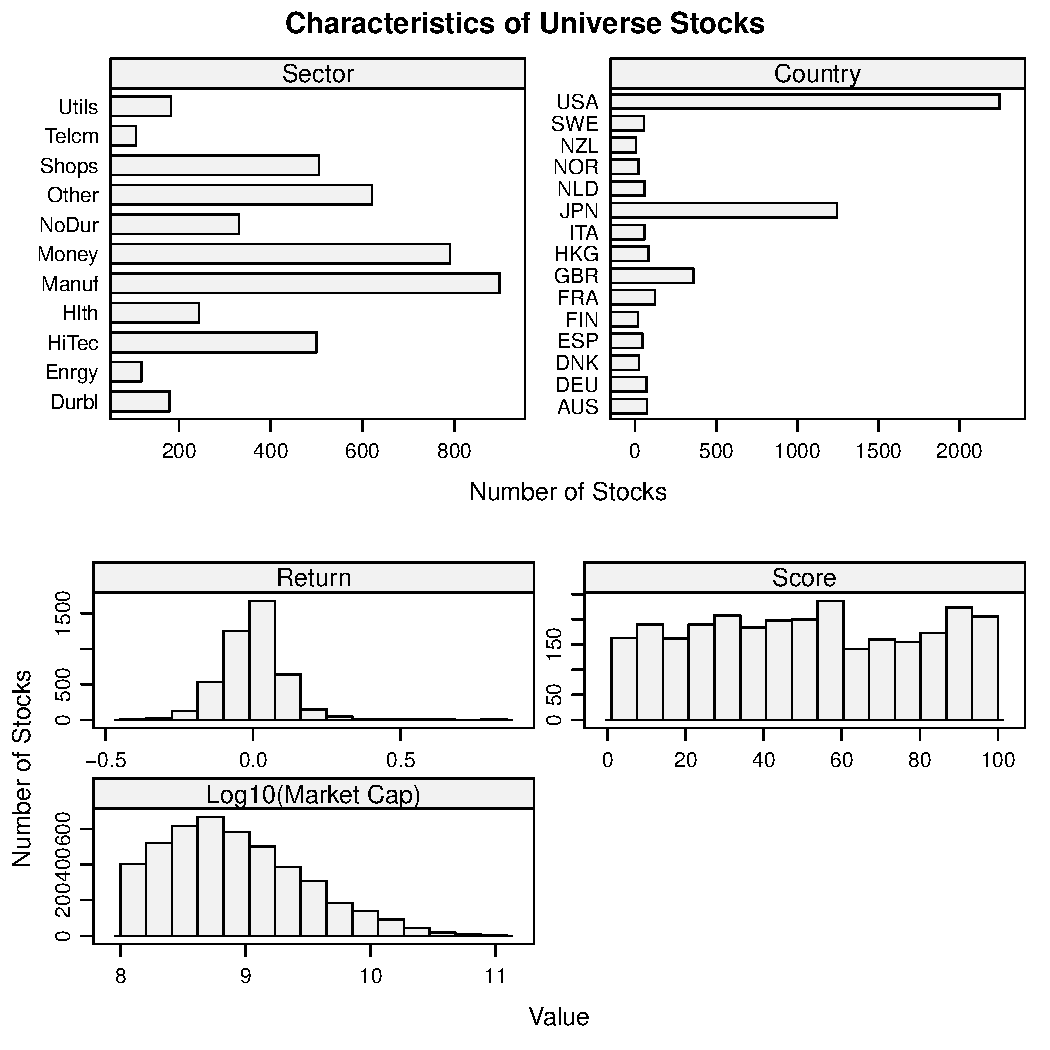
\includegraphics[width=\maxwidth]{figure/unnamed-chunk-4} 

\end{knitrout}

\end{center}
\caption{Histograms representing the makeup of the universe of stocks
  by country, sector, return, StarMine score and market capitalization
  in U.S. dollars. The complete universe of stocks is represented
  here, including both StarMine-rated stocks.}
\label{FigureStarMine}
\end{figure}




The object of our analysis is a simple long-only portfolio using the SMI score,
splitting our position equally among the 100
top-rated stocks in the universe, representing roughly the top decile of
StarMine's ratings. Figure \ref{FigureExposure} shows this portfolio's
primary exposures. The portfolio returns
19.0\\% over the following month.

Figure \ref{FigureExposure} compares this portfolio's exposures
to those of the universe. This portfolio is relatively heavily weighted in
high-tech., shopping and durable goods stocks, as well as mid-caps and
Australian stocks.

\begin{figure}
\begin{center}
\begin{knitrout}
\definecolor{shadecolor}{rgb}{0.969, 0.969, 0.969}\color{fgcolor}
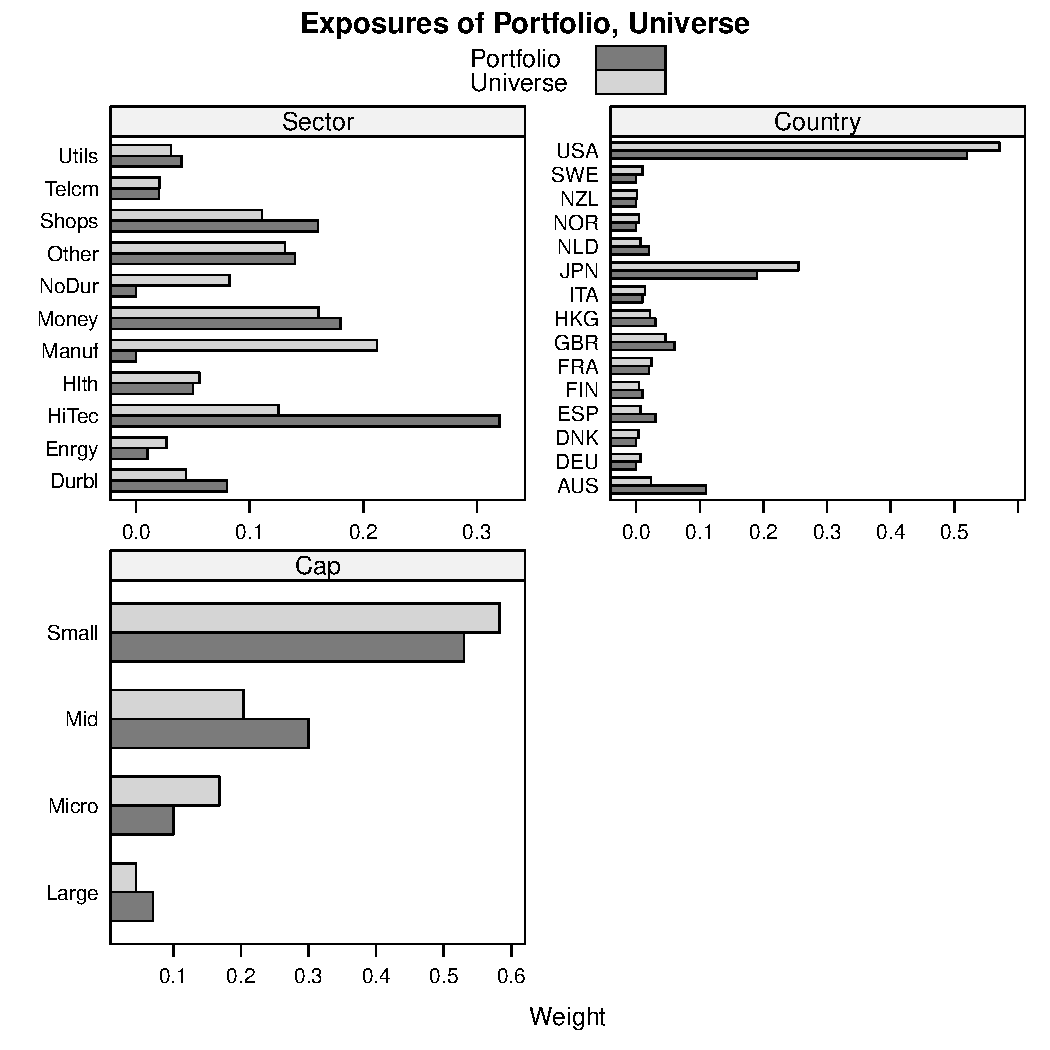
\includegraphics[width=\maxwidth]{figure/unnamed-chunk-6} 

\end{knitrout}

\end{center}
\caption{Exposures of the StarMine portfolio to sector, country and
  market cap. Also shown are exposures of an equal-weighted index of
  stocks in the rated universe.}
\label{FigureExposure}
\end{figure}

Figure \ref{FigurePerformance} shows the performance of the portfolio
next to that of various benchmarks. Compared to the S\&P, the
portfolio looks bad; compared to the equal-weighted complete universe, it looks
great. The equal-weighted return on the
rated universe also underperforms the actual portfolio.

\begin{figure}
\begin{center}
\setkeys{Gin}{height=0.4\textwidth,width=0.8\textwidth}
\begin{knitrout}
\definecolor{shadecolor}{rgb}{0.969, 0.969, 0.969}\color{fgcolor}
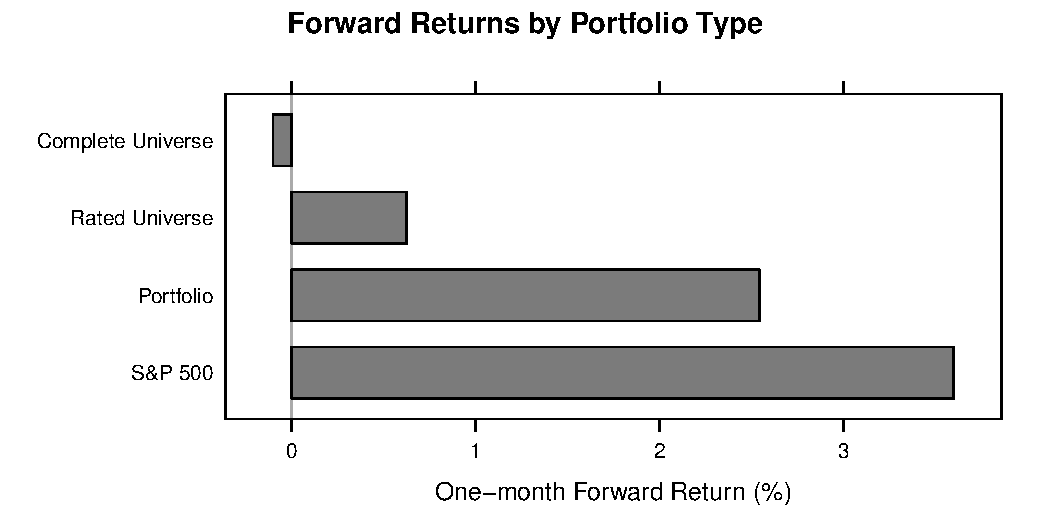
\includegraphics[width=\maxwidth]{figure/unnamed-chunk-7} 

\end{knitrout}

\setkeys{Gin}{height=0.8\textwidth,width=0.8\textwidth}
\end{center}
\caption{Performance of the StarMine portfolio compared to performance
  of various benchmarks: the S\&P 500, the equal-weighted complete
  universe, and the equal-weighted rated universe.}
\label{FigurePerformance}
\end{figure}

\section{Matching Portfolio}

In this section we give steps to build a ``matching portfolio'' that
matches the exposures of the StarMine portfolio, but holds different
stocks. We start by examining the portfolio's holdings at the time under
consideration. Associated with each stock is the set of characteristics
listed above: country, sector and market cap. Note that our method can
incorporate any number of characteristics.

We take an approach similar to that of \cite{daniel97.1} in that it measures
performance against a benchmark with the same characteristics. Ours is
more finely matched, however, pairing each holding with a
non-holding with the same characteristics. Our framework is also more
flexible, allowing for any number of characteristics.

In the sections below, we first illustrate the goal of matching and
then provide computational details. To make matches we utilize the
propensity score of \cite{rosenbaum83}, who used it to match treated
subjects to near-equivalent control subjects in an observational
study. Finally we demonstrate how matched portfolios can be used as
benchmarks, using the StarMine portfolio as an example.

\subsection{Motivation}

The simplest way to create matching portfolios is to examine the
universe of securities in the multi-dimensional characteristic
space. Figure \ref{FigurePortfolioUniverse} shows a set of
two-dimensional cross-sections by country, each showing securities by
sector and market cap. The black dots represent holdings and the gray
dots non-holdings.

For most portfolio positions, there's an abundance of very close
possible matches. A few holdings might have to reach a bit farther for
a match, such as the \$70 billion durable goods holding (Toyota Motor) on the
bottom row of the Japan panel. The nearest match with the same sector
and country is Nissan Motor (\$18 billion). Even if we allow
non-Japanese matches, the closest we can get is General Motors (\$28
billion). Thankfully, either of these is a plausible match, and most
holdings have many more possible matches.

\begin{figure}
\begin{center}
\setkeys{Gin}{height=1\textwidth,width=1\textwidth}
\begin{knitrout}
\definecolor{shadecolor}{rgb}{0.969, 0.969, 0.969}\color{fgcolor}
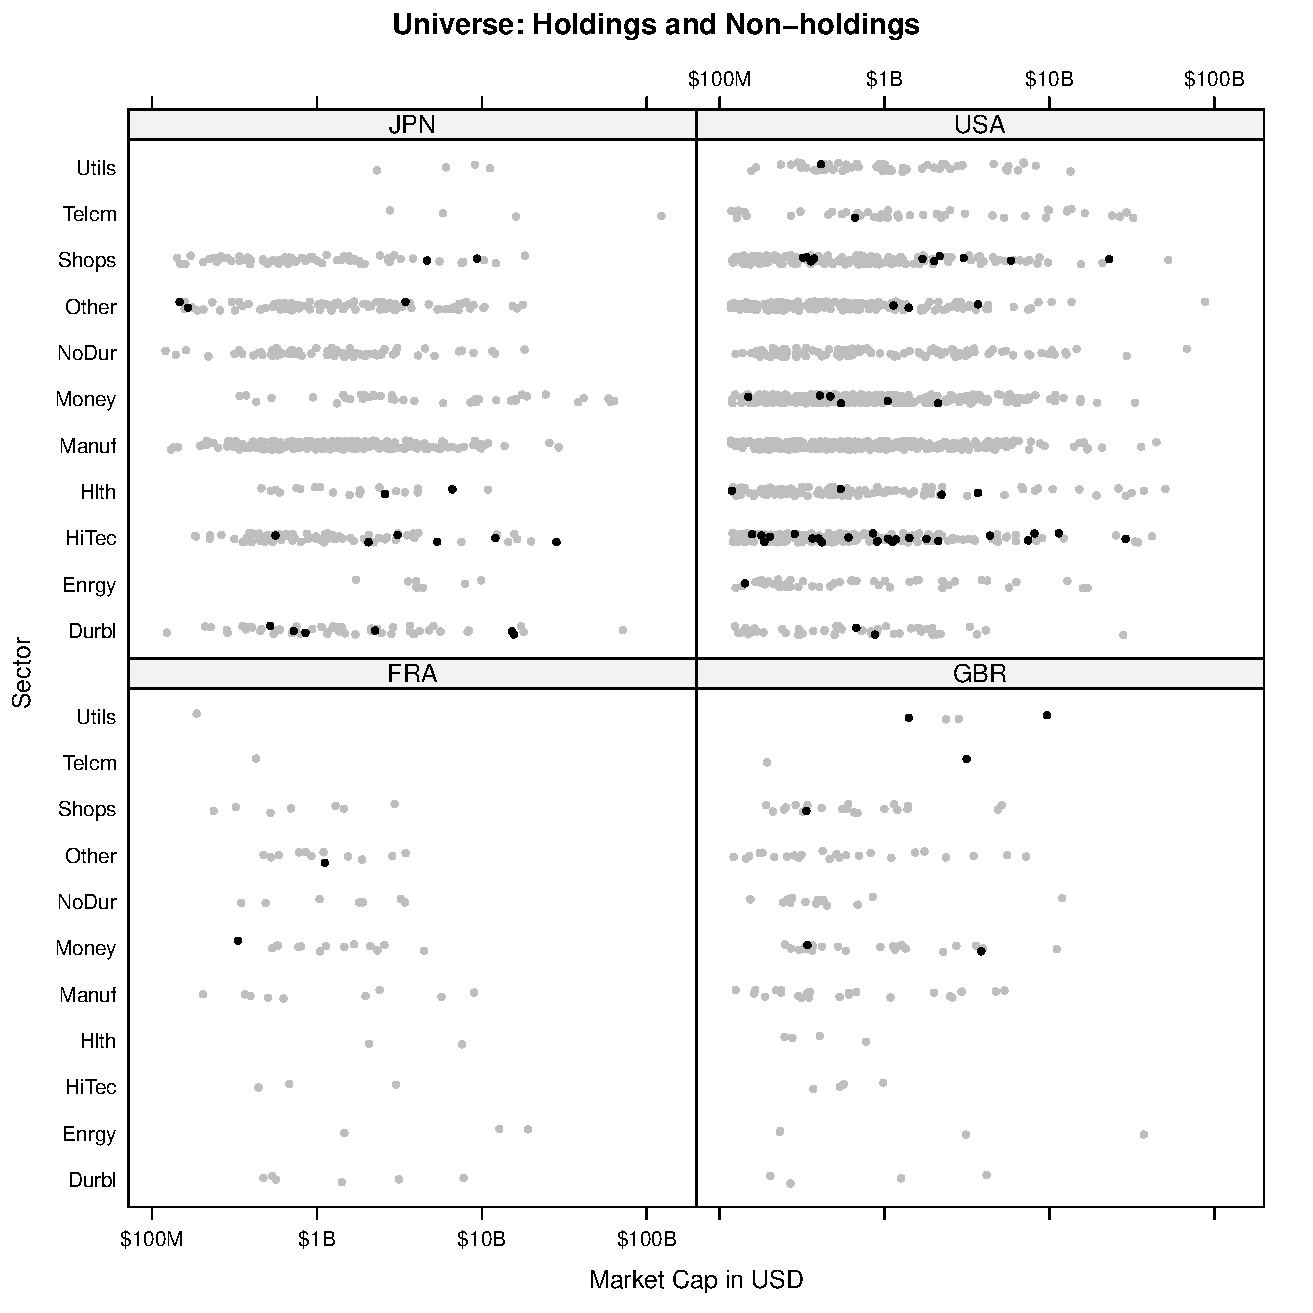
\includegraphics[width=\maxwidth]{figure/unnamed-chunk-8} 

\end{knitrout}

\setkeys{Gin}{height=0.8\textwidth,width=0.8\textwidth}
\end{center}
\caption{Cross-sections of universe stocks by market cap and
  sector. There is one panel for each of the four countries, the U.S.,
  Japan, Great Britain and Australia, with the most universe
  securities. Black dots
  are portfolio holdings and grey dots non-holdings. The vertical
  positions of the dots are jittered slightly so as to appear
  separate. Most securities have a plethora of possible matches,
  but some do not, like Toyota Motor Corp. represented by the dot in the
  lower right corner in the Japan panel. It would have to stretch all
  the way to Nissan Motor, the nearest gray dot, for a suitable match.}
\label{FigurePortfolioUniverse}
\end{figure}

\subsection{Propensity Score}

It is clear from Figure \ref{FigurePortfolioUniverse} how one would
execute matching as a visual exercise. We next discuss how to approach
matching computationally.

Matching in an arbitrarily dimensional stock characteristic space is
made challenging by the curse of dimensionality. Looking at Figure
\ref{FigurePortfolioUniverse}, one's first intuition is to find a
``nearby'' stock for each holding, under some notion of
distance. \cite{rubin73.1} and \cite{rubin73.2} investigate a variety
of matching approaches based on distance metrics, but find that these make
increasingly poor matches as the number of dimensions grows.

\cite{rosenbaum83} solve the problem with the \emph{propensity score}.
The propensity score is the estimated probability that a given
security appears in the portfolio, given only its characteristics. The
\emph{fundamental balancing property of the propensity score} shows
that matching two units based on the propensity score is sufficient,
on average, for matching them on all their characteristics.

Mathematically, define $I_i = 1$ when stock $i$ is in the original
portfolio and $I_i = 0$ otherwise, with $i \in \{1, ..., n\}$ for all
$n$ stocks in the universe. Let $X_i \in \mathbbm{R}^p$ represent the
$p$-dimensional vector of stock characteristics associated with stock
$i$. The propensity score is defined as $P(I_i = 1 | X_i)$. Typically
this probability is estimated using a logistic regression of the
binary outcome vector $I$ on the characteristics $X$ as the covariate
matrix, as described in \cite{rubin96}.

\cite{rosenbaum83} show that the propensity score is a ``balancing
score'' by the definition of \cite{dawid79}: a single-dimensional
value that acts to ``balance'' the values of the entire vector
$X_i$. Statistically, this
means $I_i \perp X_i | b(X_i)$; i.e., there is independence between
$I_i$ and $X_i$ given the balancing score $b(X_i)$. In words, this
means that if we match stocks to each other using only the estimated
probabilities $b(X_i) = \hat{P}(I_i = 1 | X_i)$, then we have
effectively matched them on the basis of all the characteristics. A
multidimensional problem is thus reduced to one dimension.

Estimating a propensity score model for the StarMine portfolio, we
obtain the fitted coefficients in Table
\ref{TablePropensityScore}. The sector and country variables are swept
out as a set of 1/0 indicators with an excluded level for each:
``AUS'' for the country indicators and ``Durbl'' for the
sectors. Indicators corresponding to countries unrepresented in the
portfolio are mathematically $-\inf$ and are excluded from the
table.

The model's positive coefficients correspond to characteristics
to which the portfolio is over-exposed relative to the universe. All
of the country indicators are negative, showing exposure to the
excluded level, Australia. Likewise, the positive high-tech
coefficient indicates exposure to that sector.

% latex table generated in R 3.0.1 by xtable 1.7-1 package
% Mon Aug 05 11:27:56 2013
\begin{table}[ht]
\centering
\begin{tabular}{rrrrr}
  \hline
 & Estimate & Std. Error & t value & Pr($>$$|$t$|$) \\ 
  \hline
(Intercept) & -0.9376 & 0.5341 & -1.76 & 0.0793 \\ 
  1(country = ESP) & -0.2853 & 0.6762 & -0.42 & 0.6731 \\ 
  1(country = FRA) & -2.3570 & 0.7093 & -3.32 & 0.0009 \\ 
  1(country = GBR) & -1.6506 & 0.4854 & -3.40 & 0.0007 \\ 
  1(country = HKG) & -1.6870 & 0.6098 & -2.77 & 0.0057 \\ 
  1(country = ITA) & -2.3288 & 0.9441 & -2.47 & 0.0137 \\ 
  1(country = JPN) & -2.5422 & 0.3942 & -6.45 & 0.0000 \\ 
  1(country = NLD) & -0.5848 & 0.7772 & -0.75 & 0.4519 \\ 
  1(country = USA) & -2.3038 & 0.3535 & -6.52 & 0.0000 \\ 
  1(sector = Enrgy) & -2.0115 & 0.9476 & -2.12 & 0.0339 \\ 
  1(sector = HiTec) & 0.4691 & 0.3677 & 1.28 & 0.2021 \\ 
  1(sector = Hlth) & -0.5659 & 0.4951 & -1.14 & 0.2532 \\ 
  1(sector = Money) & -0.8568 & 0.4038 & -2.12 & 0.0339 \\ 
  1(sector = Other) & -0.9720 & 0.4196 & -2.32 & 0.0206 \\ 
  1(sector = Shops) & -0.3487 & 0.4015 & -0.87 & 0.3852 \\ 
  1(sector = Telcm) & -1.0009 & 0.7173 & -1.40 & 0.1630 \\ 
  1(sector = Utils) & -0.8703 & 0.5919 & -1.47 & 0.1416 \\ 
  1(cap = Small) & 0.4362 & 0.3019 & 1.44 & 0.1486 \\ 
  1(cap = Mid) & 1.1850 & 0.3282 & 3.61 & 0.0003 \\ 
  1(cap = Large) & 1.1699 & 0.4536 & 2.58 & 0.0100 \\ 
   \hline
\end{tabular}
\caption{Coefficients from the fitted logistic regression for propensity score using indicator variables from the StarMine portfolio.} 
\label{TablePropensityScore}
\end{table}



\subsection{Computation}

Next we use the propensity score to match holdings to nearby
non-holdings with similar propensity scores. There are several ways of
finding matches, and \cite{abadie06} provides a nice review of the
possibilities. The simplest, proposed by \cite{cochran73}, is
\emph{nearest-available matching}, sometimes called ``greedy
matching.''

For each portfolio holding $i \in \{1, ..., n\}$,
\begin{enumerate}
\item Find the security $j$ that minimizes the absolute difference in
  propensity scores $|b(X_i) - b(X_j)|$. Add it to the matched
  portfolio with the same weight as holding $i$.
\item Remove security $j$ from the universe of possible matches. This
  is to ensure that matched holdings are selected \emph{without
  replacement}. This ensures that no match is given double weight in
  the matched portfolio.
\end{enumerate}

Greedy matching is imperfect, and one could benefit from
rearranging matches optimally. The gains from this would be small in
our case because the size of our universe relative to the
portfolio ensures a large reservoir of possible matches.

The propensity score's balancing behavior is a distributional
property. Balance is realized asymptotically, not at
the level of the individual match. While individual matches may not
appear matched, the entire matched portfolio's exposures usually come
close to matching the original's. For this reason we do not report any
specific stocks' matches, but rather focus on the exposures of the
entire matched portfolio.

To execute the matching procedure, we use the ``MatchIt'' package of
\cite{matchit.pkg} and explained in detail in
\cite{matchit.paper}. Figure \ref{FigurePortfolioMatchExposure}
compares the exposures of the original portfolio with those of the
propensity score-matched portfolio. There are no points of significant
disagreement. The matched portfolio has nearly exactly the same
characteristics as the original.

\begin{figure}
\begin{center}
\begin{knitrout}
\definecolor{shadecolor}{rgb}{0.969, 0.969, 0.969}\color{fgcolor}
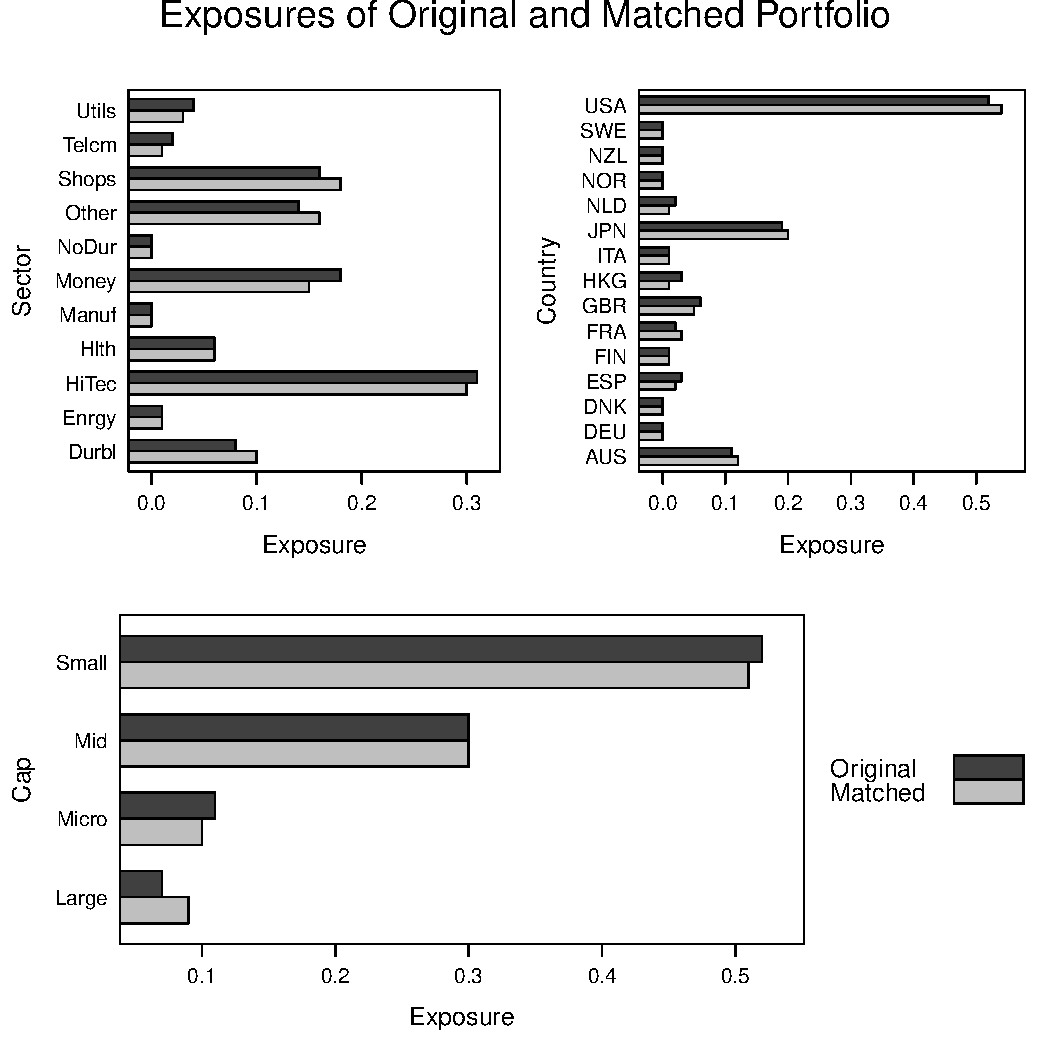
\includegraphics[width=\maxwidth]{figure/unnamed-chunk-10} 

\end{knitrout}

\end{center}
\caption{Bar plots comparing the exposures of the original StarMine
  portfolio (light grey) to those of the matched portfolio (dark grey)
  comprised of different but similar securities. The exposures match
  closely in every characteristic under consideration.}
\label{FigurePortfolioMatchExposure}
\end{figure}

\subsection{Performance}




After we have found a matching portfolio, outperformance
can be expressed as a simple difference of returns from the original
to the matched portfolio. Mathematically, this can be expressed as
$$ \sum_i w_i r_i - \sum_i \tilde{w}_i r_i, $$
where $r_i$ represents the forward return on security $i$, $\{ w_i \}$
the portfolio weights of securities in the original portfolio and $\{
\tilde{w}_i \}$ the portfolio weights of securities in the matched
portfolio. Here $i$ indexes all stocks in the universe, $i \in \{1,
..., n\}$, so that most $w_i = 0$.

For the StarMine portfolio, the matching portfolio attains a return of
24.94\\%
versus a return of 19.0\\% for the original
portfolio, so the portfolio slightly outperforms. The simple
weighted average of the universe yields a somewhat higher
outperformance, but this is narrowed when matching portfolios are used
as benchmarks. This implies that some of the StarMine portfolio's
total performance comes from favorable sector, country and market cap
bets.

\section{Random Portfolios}

Instead of creating a single matched portfolio, consider creating
1,000. Consider Figure \ref{FigurePortfolioUniverse}. Note how each
stock in the target portfolio has many possible matches. Yet these
matches may not all tell the same story. Inevitably, some will have
higher return than others. The set of returns on these portfolios,
each containing a different set of matched securities, provides some
measure of uncertainty in our performance measurement. Each matched
portfolio provides an estimate of ``alpha'' as the difference between
its return and the original portfolio's return. This yields a
distribution for ``alpha.''

The relative position of the original portfolio's return among the
matched portfolios' returns is the primary quantity of interest. The
relative position allows us to conduct a nonparametric hypothesis test
of the claim that $alpha = 0$ based on the empirical distribution of
matching portfolio returns.

Our approach to random portfolios is distinguished by its emphasis on
matching portfolios. \cite{burns04} and \cite{dawson03} use a similar
procedure, but do not require the random portfolios to be matched to
the original. As such, their random portfolios reflect the makeup of
the universe more than the makeup of the target portfolio, and could
have widely varying cap, sector and country exposures. We propose a
stricter framework: limiting portfolios to those within a certain
distance from the original.

\subsection{Procedure}




Before we can sample portfolios, we need some guidelines on how far a
matching portfolio is allowed to be from the original. The tradeoff is
between quality and quantity of the matched portfolios. The closer we
require portfolios to be matched, the fewer of them available. The
simplest approach is to set a treshold in the propensity score 
difference allowed for an individual stock to be considered a match,
as done by \cite{rosenbaum85}. We consider two such thresholds, 0.005
and 0.05 (recall that this is relative to the space of propensity scores, on
$(0,1)$) in the two figures below.

Next we must decide how we will sample a non-holding from among each
holding's matches. To do this, we must induce a distribution among the
matches. The simplest possibility is to choose a matching non-holding
uniformly at random, and that is the practice we adopt below. Also
note that not all holdings have matches within a specified threshold. For
these, the nearest available is selected, non-randomly. Hence the
procedure collapses to simple matching as the threshold nears zero and
collapses to \cite{burns04}-style random portfolios as the threshold
grows to 1. Finally, the matches are sampled sequentially,
one holding at a time.

To recap, for our experiment we build $K = 100$ random portfolios as follows:

\begin{enumerate}
\item For each portfolio holding, define a ``match'' as any
  non-holding within a threshold distance of the holding.
\item If the holding has at least one match, choose a
  non-holding randomly from the set of matches. If the holding has
  zero matches, simply pick the nearest available
  non-holding.
\item Repeat until all portfolio holdings have matches.
\end{enumerate}

Figure \ref{FigureRandomPortfolioExposure} shows the sector exposures
of 100 random portfolios under two different propensity score
difference thresholds, 0.005 and 0.05. For each portfolio we also
computed ``total absolute bias,'' defined as the sum of the absolute
differences in sector exposures between the original and matched
portfolio. Quintiles of total absolute bias appear on the X axis,
demonstrating that the 0.005
threshold leads to somewhat less bias than the 0.05 threshold. The
tick marks on the Y axis correspond to the sector exposures of the
original portfolio.

Since most of the random portfolios' sector exposures line up closely
with the original's, it is clear that the random portfolio procedure
is indeed producing matched portfolios. There is visibly less bias
with the tighter threshold, though the difference is moderate. For the
returns results related in the following sections we use the
0.005-threshold random portfolio collection.

\begin{figure}
\begin{center}
\setkeys{Gin}{height=1\textwidth,width=1\textwidth}
\begin{knitrout}
\definecolor{shadecolor}{rgb}{0.969, 0.969, 0.969}\color{fgcolor}
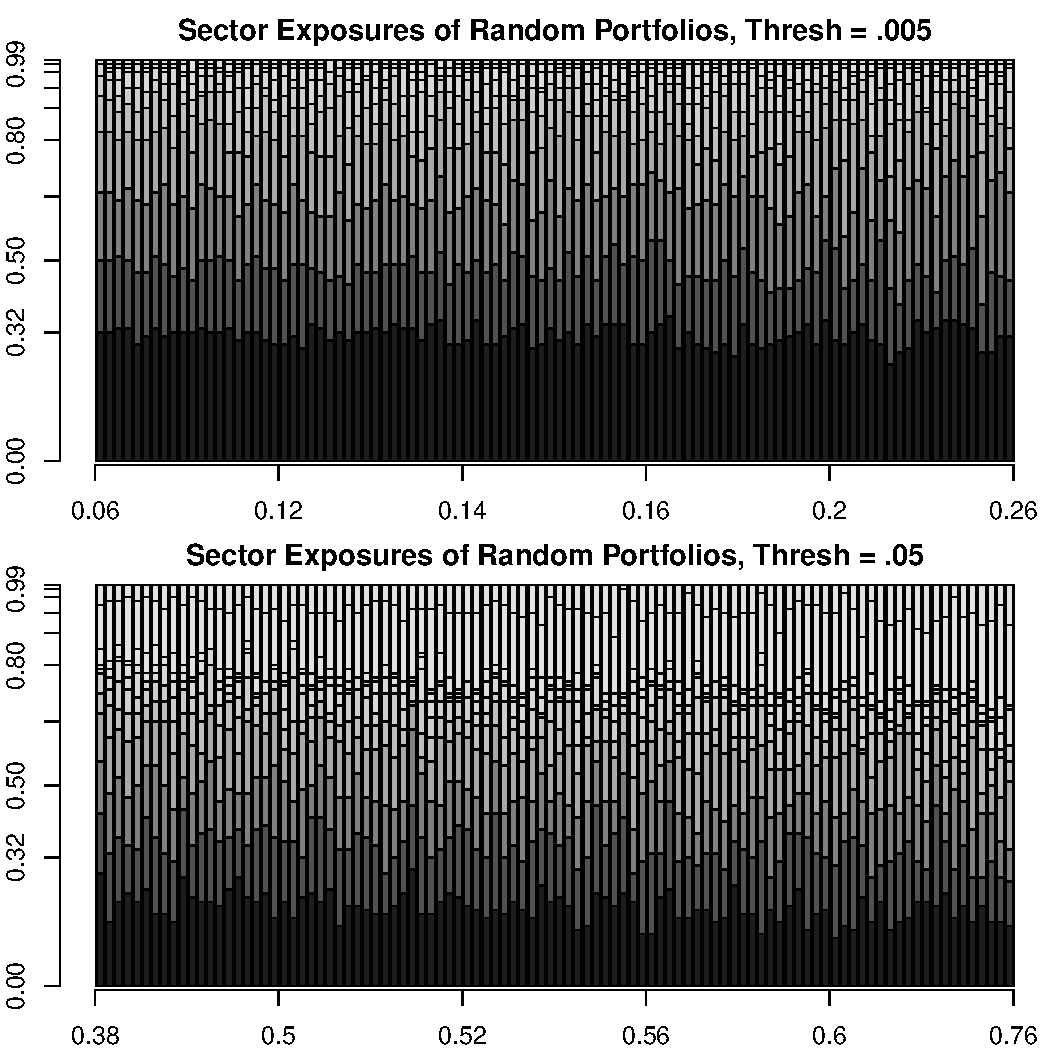
\includegraphics[width=\maxwidth]{figure/unnamed-chunk-13} 

\end{knitrout}

\setkeys{Gin}{height=0.8\textwidth,width=0.8\textwidth}
\end{center}
\caption{This figure shows the distribution of sector exposures of 100
  random portfolios. The Y axis has tick marks at the cumulative
  exposures of the original portfolio. The X axis reflects quintiles
  in the distribution of absolute bias across the random
  portfolios. The portfolios are sorted from left to right in
  ascending order on total absolute bias, so the leftmost portfolios
  are closest to the original and the rightmost are farthest. There is
  a slight gain in closeness evident in the set of matching portfolios
  based on a tighter propensity score bound.}
\label{FigureRandomPortfolioExposure}
\end{figure}

\subsubsection{Results}




We next compare the returns enjoyed by the random, matching portfolios
to those of the original. Figure \ref{FigureRandomPortfolio} shows the
distribution of matched portfolio returns along with a vertical line
representing the original portfolio's return. The StarMine portfolio
outperforms 35.0\\% of the
random, matching portfolios. This provides some evidence for
outperformance of the StarMine portfolio, but not enough to achieve
statistical significance.

\begin{figure}
\begin{center}
\begin{knitrout}
\definecolor{shadecolor}{rgb}{0.969, 0.969, 0.969}\color{fgcolor}
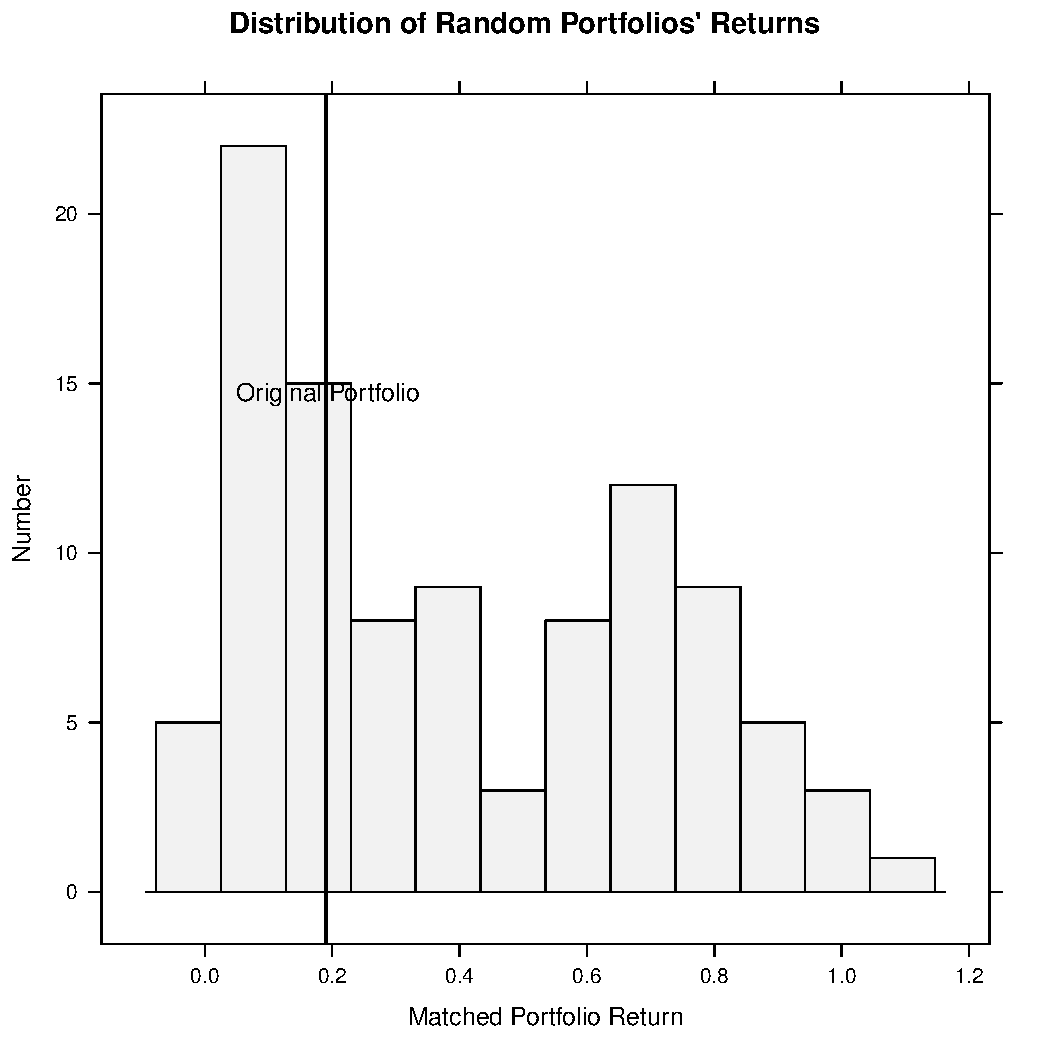
\includegraphics[width=\maxwidth]{figure/unnamed-chunk-15} 

\end{knitrout}

\caption{Histogram showing the returns of random, matched portfolios
  for the StarMine data. The thick vertical line represents the return
  realized by the StarMine decile portfolio. It stands at the
  35.0\\% percentile of the
  random returns.}
\label{FigureRandomPortfolio}
\end{center}
\end{figure}

\section{Long-Short Portfolios}

One great advantage of the matching portfolio framework is that it
effortlessly allows for different weighting strategies, such as
non-equal-weighted long portfolios and long-short
portfolios. Managers have struggled to find decent
benchmarks for long-short portfolios. \cite{jacobs99} write that there
are no inherent benchmarks suitable for a long-short portfolio,
besides the return on cash. In our framework, we simply create a
matching portfolio, where each stock gets the same as its matching
stock holds in the original portfolio.

In this section we build a long-short version of the StarMine
portfolio based on the StarMine score. We then describe how to
construct matching portfolios when the portfolio is not
equally-weighted long using the ``generalized propensity'' score due to
\cite{imai04}, \cite{hirano04} and \cite{lu01}. Finally, we sample
random portfolios and compare the performance results to other
measures.




For the tests in this section we create a long-short portfolio
based on the StarMine score. We divide the long position equally between
stocks among the top 10\% of StarMine scores and the short position
between stocks in the bottom 10\%. The total short position is 75\% of
the long position, creating a 100/75 long-short portfolio.

The long and short exposures of this portfolio are given in Table
\ref{FigureLSMatchExposure}. Overall, the portfolio returns
-44.8\\%.




Some of the mechanics of matching must change. Previously we followed
the Rubin Causal Model by analogizing a stock's inclusion in the
portfolio to what \cite{rosenbaum83} call a ``treatment effect'' (see
Appendix). The variable $I_i$ associated with this treatment is
defined to be one when stock $i$ is in the portfolio and zero
otherwise. Matching on the propensity score $P(I_i = 1 | X_i)$ yields
matched stocks with the same probability of inclusion in the
portfolio, which guarantees exposure balance between the original and
matched portfolio. The definition of this probability depends on
the treatment indicator $I_i$ being a binary random variable.

But in a long-short portfolio, inclusion takes two forms: long and
short. For a portfolio with unequal weights, inclusion can refer to
any nonzero weighting. Generally, the treatment is best
described as a continuous random variable, where $I_i = w_i$, stock
$i$'s weight in the original portfolio. Of course, since $I_i$ is no
longer binary, the propensity score method cannot be applied directly.

To match with continuous weights, we employ the ``generalized
propensity score'' of \cite{imai04}. In this approach, we fit a model
for $b(X_i) = E[I_i | X_i]$ as a function of $X_i$. The most popular choice
is a linear regression, which writes $\hat{b}(X_i) = \hat{\beta}' X_i$
for a fitted coefficient $p$-vector $\hat{\beta}$. Both \cite{imai04}
and \cite{hirano04} show that the expected value
acts as a balancing score, ensuring $I_i \perp X_i | b(X_i)$. This
means that we can create a characteristic-matched portfolio by
matching on the univariate score $b(X)$, just as we can for the
propensity score in the binary treatment case.

Next we fit $\hat{b}(X_i)$ using a linear regression of the weights
$I_i = w_i$ on the covariates $X_i$ representing the same set of
indicator variables as before. The $R^2$ from the fit is poor, only
0.08. Yet \cite{lu01} has shown
that even a poor fit for the propensity score can lead to
well-balanced matches.

To find matches, we adopt much the same procedure as we did in the simple
propensity score case, with the added tweak that matched non-holdings
receive the weight given their original holding. The propensity score
procedure for the equal-weighted case can be considered a sub-case of the
current methodology.

\begin{enumerate}
\item Match each holding $i$ to a non-holding $\mathcal{P}(i)$ using the
  estimated generalized propensity score $\hat{\beta}$.
\item Assign non-holding $\mathcal{P}(i)$ a weight in the matched
  portfolio equal to $i$'s weight in the original portfolio; i.e.,
  $\tilde{w}_{\mathcal{P}(i)} = w_i$.
\item Continue matching until every holding has a matching non-holding.
\end{enumerate}

In our case, Figure \ref{FigureLSMatchExposure} shows
the long and short exposures of the original and matched
portfolios. We can see that both the long and short bets in the
original portfolio line up very nicely with the matched portfolio's.

The matched portfolio returns 11.6\\%
compared with -44.8\\% for the original
portfolio. This suggests that the StarMine long-short portfolio
exhibits some stock-picking ability; its returns are more than can be
explained by its sector, country and market cap bets.

\begin{figure}
\begin{center}
\begin{knitrout}
\definecolor{shadecolor}{rgb}{0.969, 0.969, 0.969}\color{fgcolor}
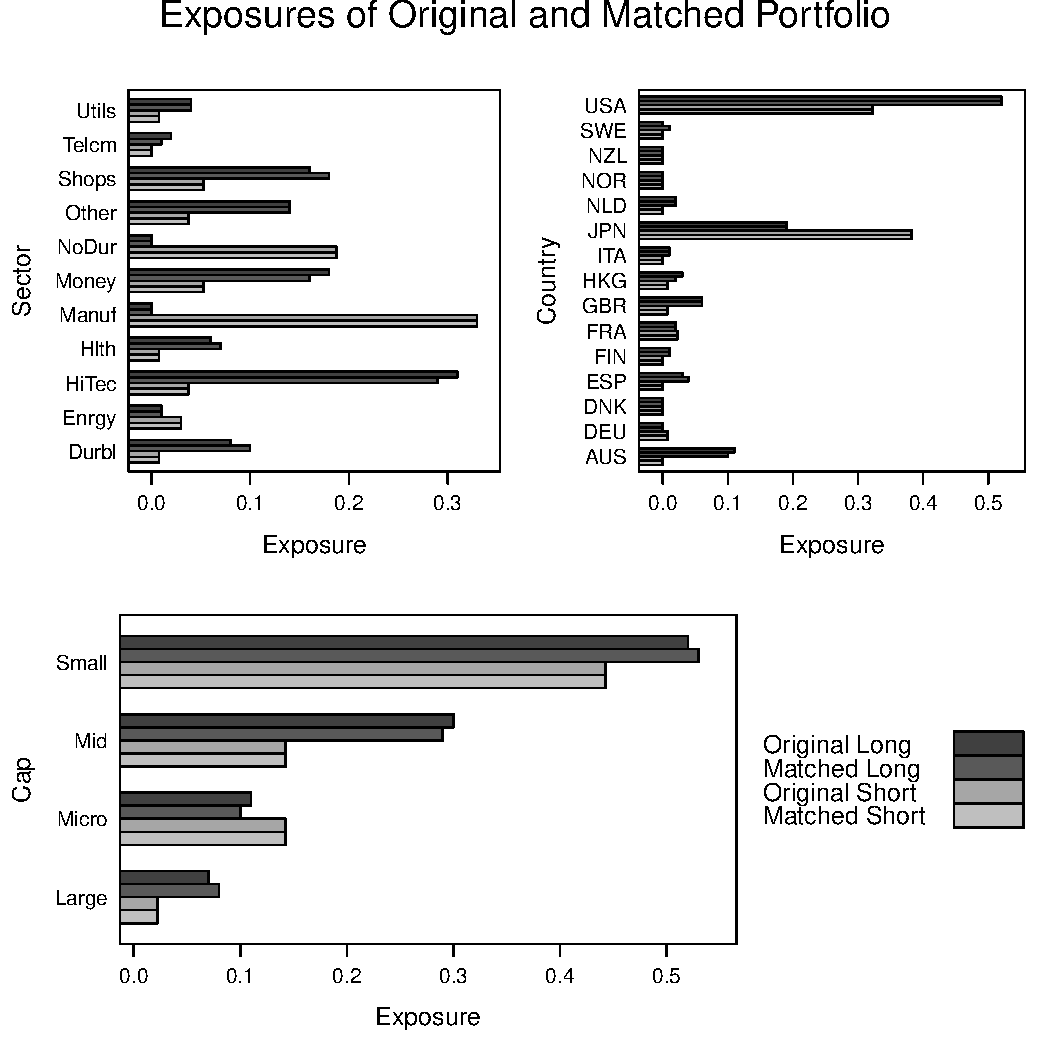
\includegraphics[width=\maxwidth]{figure/unnamed-chunk-18} 

\end{knitrout}

\end{center}
\caption{The long and short exposures of the original long-short
  StarMine portfolio and the portfolio matched to it using the
  generalized propensity score. Both the long and short exposures line
  up very nicely.}
\label{FigureLSMatchExposure}
\end{figure}

We can form random matching portfolios much the same way we did using
the simple propensity score. We simply define a threshold distance for
the generalized propensity score, within which every non-holding is
taken to be a match. The scale of the propensity score is the same as
the scale of the weights it models. In our case, we find a threshold
of 0.0001, a single basis point, to lead to high-quality matches
without sacrificing diversity.




The returns of the matching portfolios are shown in the histogram in
Figure \ref{FigureLSRandomPortfolio}. Since the original portfolio's
return falls at the 2.0\\%
percentile of the random portfolios' returns, it turns out to be a
little worse than we thought. We cannot reject the hypothesis that the
stock-picking ability is zero.

\begin{figure}
\begin{center}
\begin{knitrout}
\definecolor{shadecolor}{rgb}{0.969, 0.969, 0.969}\color{fgcolor}
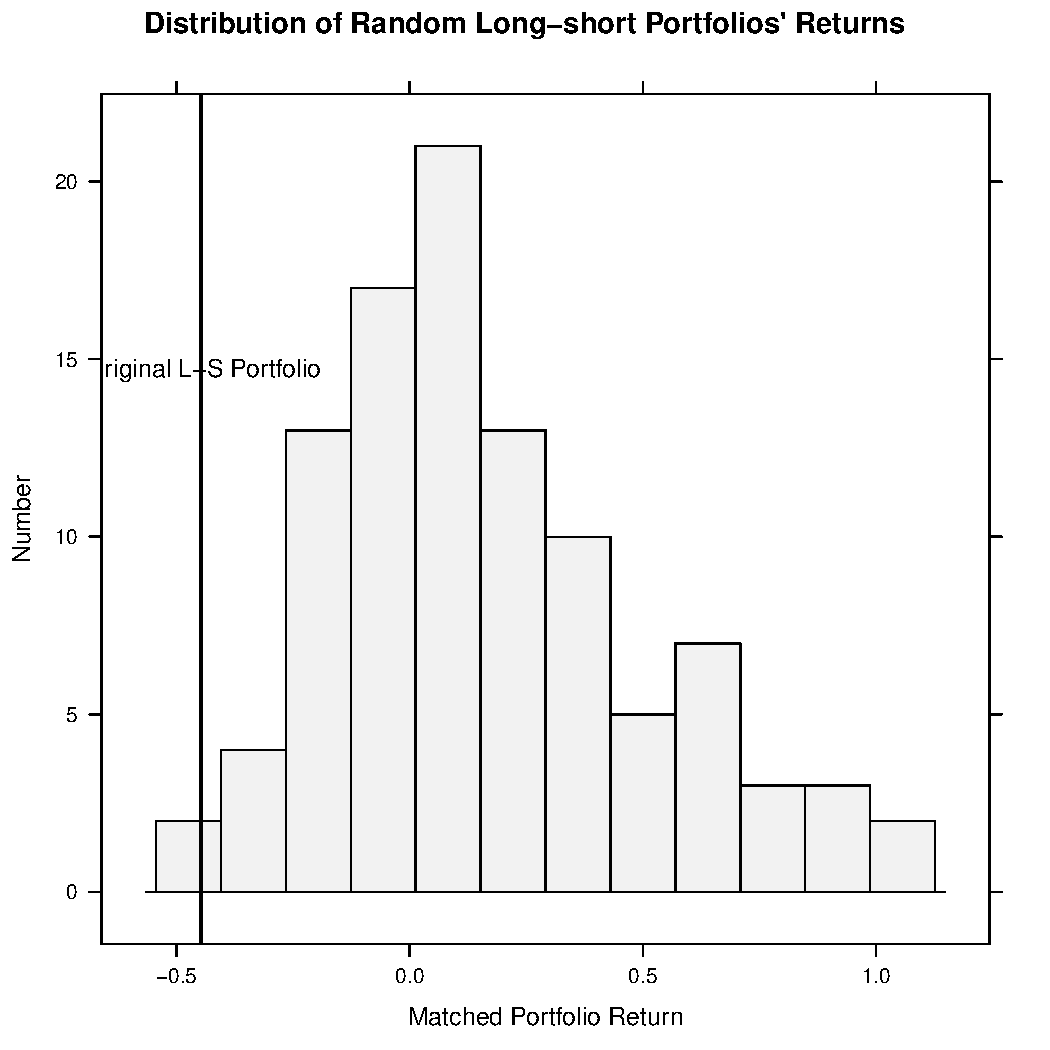
\includegraphics[width=\maxwidth]{figure/unnamed-chunk-20} 

\end{knitrout}

\caption{Histogram showing the returns of random portfolios matched to
  the long-short StarMine portfolio. The thick vertical line
  represents the return realized by the StarMine decile portfolio. It
  stands at the 2.0\\%
  percentile of the random returns, suggesting that the StarMine
  portfolio's excess return is indeed due to stock-picking ability.}
\label{FigureLSRandomPortfolio}
\end{center}
\end{figure}

\begin{figure}
\begin{center}
\setkeys{Gin}{height=0.5\textwidth,width=0.8\textwidth}
\begin{knitrout}
\definecolor{shadecolor}{rgb}{0.969, 0.969, 0.969}\color{fgcolor}
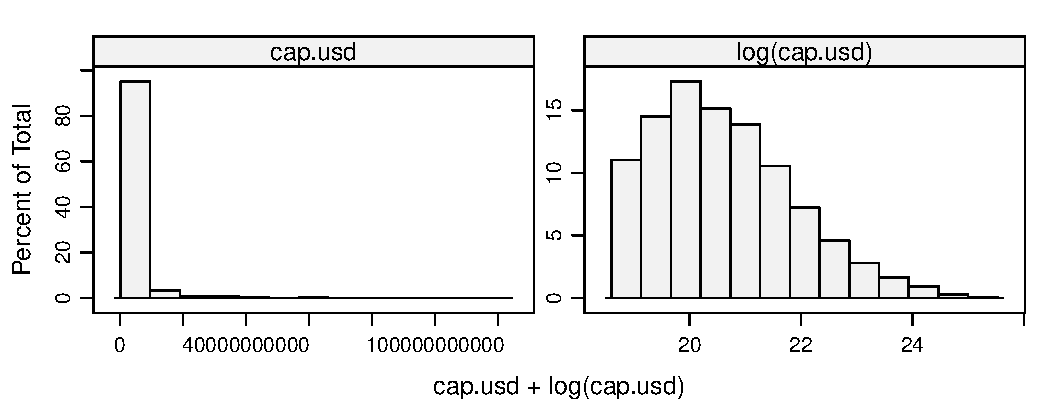
\includegraphics[width=\maxwidth]{figure/unnamed-chunk-21} 

\end{knitrout}

\setkeys{Gin}{height=0.8\textwidth,width=0.8\textwidth}
\end{center}
\caption{Comparisons of returns from the actual StarMine portfolio
  with returns from benchmark portfolios: the S\&P 500; the simple
  average return of rated universe stocks; the average return of
  propensity score-based matching long-only portfolios; the
  long-short portfolio constructed based on the SMI score; and the
  average return of matching long-short portfolios.}
\label{FigureReturnComparison}
\end{figure}

\section{Conclusion}

Our method evaluates performance by comparing the returns of the target
portfolio to a counterfactual portfolio with the same characteristics
but different holdings. This comparison isolates a manager's
stock-picking ability from the effect of characteristic exposures.
We have shown that the propensity score provides a flexible and precise means of
constructing matching portfolios. Our methodology extends naturally to
creating matching portfolios under any weighting scheme.

\bibliography{matching}

\end{document}

\section{Appendix}

\subsection{Matching}

In the following sections we describe three types of portfolio matching:

\begin{itemize}
\item \emph{Multivariate}, based on a distance metric between securities'
  market factors.
\item \emph{Categorical matching}, in which we attempt to match a
  security's categorical factors -- e.g., country, sector -- exactly.
\item \emph{Propensity scoring}, in which a high-dimensional market
  factor space is collapsed to a single dimension on which matching is
  performed.
\end{itemize}

\subsubsection{Mahalanobis Distance Metric}

Figure \ref{FigurePortfolioUniverse} suggests that we should
match each holding to a nearby holding. But what do mean by distance
in a space of market factors?

For the purpose of this section suppose that all market factors are
numeric -- that is, continuous values rather than categories. In later
sections we address how to handle categorical values. For now, assume
security $i$'s $p$ market factors can be represented as
$M_i \in \mathbbm{R}^p$ for $i \in \{1, ..., N\}$, where $N$ is the
number of securities in the
universe. Further suppose $\mu = E[M_i]$, the mean of $M_i$, and
$\Sigma = Cov(M_i)$, the covariance matrix of the market factors.

A simple distance option would be the Euclidean distance measure
\begin{equation}
D(M_i, M_j) = \sqrt{(M_i - \mu)' (M_i - \mu)},
\end{equation}
but this would not discount the effect of highly correlated
market factors. For instance, suppose that we seek to match on
liquidity, market cap and book-to-market ratio. Liquidity and market
cap are highly correlated, but neither is correlated with
book-to-market ratio. Euclidean distance would have the effect of
weighting the first two factors equally.

Instead we use the \emph{Mahalanobis distance} of
\cite{mahalanobis36} and recommended by \cite{cochran73} in numerous
matching studies. The Mahalanobis distance is similar to Euclidean
distance, but shifts directions based on the covariance matrix. The
Mahalanbois distance between securities $i$ and $j$ is defined as
\begin{equation}
D(M_i, M_j) = \sqrt{(M_i - \mu)' \Sigma^{-1} (M_i - \mu)}.
\end{equation}
In practice $\Sigma$ is usually replaced by $\hat{\Sigma}$, the
estimated covariance matrix from the observed pattern of market
factors.

\subsubsection{Categorical Matching}

The previous section addresses matching for continuous, numeric
variables. For matching on categorical variables, \cite{cochran73}
points out two reasonable approaches:

\begin{itemize}
\item Populate a set of 0/1 indicator variables representing the
  categories. Treat these as numeric variables in the distance
  measure. Because we have 11
  sectors, 15 countries and a
  single market cap variable, this amounts to a total of $p = $
  27
  dimensions in the market factor space.
\item Force matching on categorical variables to be exact. That is,
  only match Japanese tech companies to other Japanese tech companies.
\item Perform some combination of the above.
\end{itemize}

The downside with the second approach is that if there are many market
factors, there may be few or no matches available for some
holdings. The downside with the first approach, as pointed out by
\cite{rubin73.1}, is that categorical values can distort a Mahalanobis
distance metric in unforeseeable ways. For the results in this section
we have few enough categorical variables that we perform exact
matching on sector and country.

\subsubsection{Transformations}

The distance metric is best-behaved when the variables approximate
multivariate normality. We take the log of the market cap variable to
obtain near-normality. Figure \ref{FigureTransformation} shows
the histogram before and after taking the log. If we do not normalize,
the estimated variance will be inflated. Consequently match quality
would suffer among small caps, since a difference of \$100 million
is insignificant on the scale of billions.

\begin{figure}
\begin{center}
\setkeys{Gin}{height=0.4\textwidth}
\begin{knitrout}
\definecolor{shadecolor}{rgb}{0.969, 0.969, 0.969}\color{fgcolor}
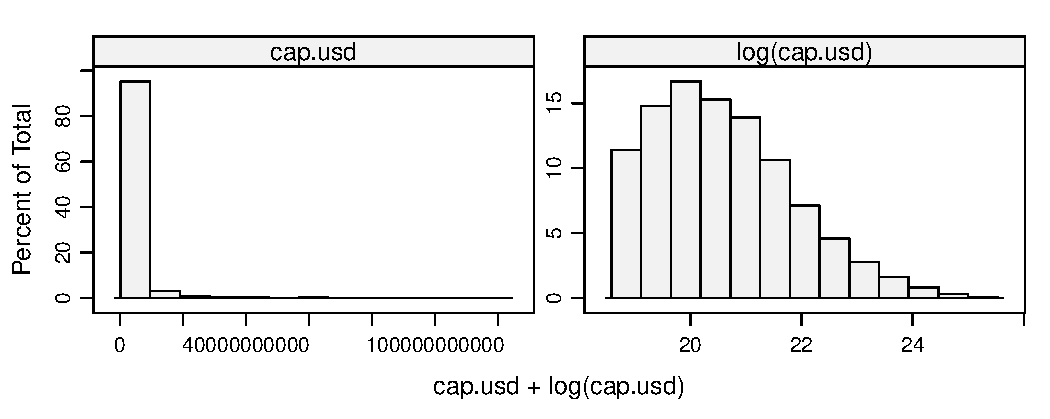
\includegraphics[width=\maxwidth]{figure/unnamed-chunk-22} 

\end{knitrout}

\caption{Two histograms of market caps of universe stocks: one on the
  native scale and one on the log scale.}
\label{FigureTransformation}
\end{center}
\end{figure}
\setkeys{Gin}{height=0.8\textwidth}

Our ordering of the rows by market cap is not critical. Though it does
improve a few matches, the vast majority will be satisfactory regardless of
ordering. There are also several algorithms that execute ``trades'' after the
initial assignment to find even better matches. That way, if Toyota
initially has to settle for a sub-par match, it would be allowed to
trade its match to obtain Nissan. Finding trades like this
is a combinatorial optimization problem and can greatly
increase computational time. One popular choice is the ``GenMatch''
algorithm of \cite{diamond05}.

\subsubsection{Propensity Score}

With large numbers of market factors, matching becomes increasingly
challenging. \cite{rubin74} showed that quality decays as the number of
dimensions grows large. The matches become more and more dependent on
the distance metric used. 

For high-dimensional spaces of market factors, matching can be eased
by \emph{balancing scores}, a concept introduced by
\cite{dawid79}. First define
$$ P_i = 1 \{ \textrm{Security }i\textrm{ is in portfolio} \}, $$,
the indicator variable valued 1 if the security is in the portfolio
and 0 otherwise.
A balancing score $b(M_i)$ is a fucntion with the property that
$$ M_i \perp P_i | b(M_i) $$
It follows that if two securities share the same balancing score $b =
b(M_i) = b(M_j)$, then on average $M_i | P_i = 0 \sim M_i | P_i =
1$. In other words, the two securities share have the same
distribution of market factors. The implication for matching is that
it is sufficient to match on the
value of the balancing score $b(M_i)$ instead of the complete
multivariate distance above. In words, the balancing score is a complete
univariate summary of a vector of covariates.

\cite{rosenbaum83} proved that the propensity score is the coarsest
balancing score possible. The \emph{propsensity score} is defined as
$b(M_i) = P(P_i = 1)$. In practice, the true propensity score is
replaced by an estimated version $\hat{P}(P_i = 1)$, most commonly
modeled through a logistic regression as explained in \cite{rubin96}.

One advantage of the propensity score is that it handles categorical
variables somewhat more gracefully, allowing them to enter the
logistic regression as a collection of indicator variables.

\subsection{Performance Attribution}

% Contribution analysis: contribution/attribution.

\subsubsection{Factset Three-factor Decomposition}

There are many empirical ways to decompose a portfolio's outperformance into
components involving stock characteristics. We provide one popular method
below that breaks excess return into an ``allocation effect,'' ``selection
effect'' and ``interaction effect.''

Suppose there is a discrete stock characteristic with $G$ levels (e.g.,
sector). A portfolio is invested with weights $\{w_{p, i} \}_{i = 1, \ldots,
G}$ in the $G$ levels. Let $r_{p, i}$ denote the return of holdings in the
$i^{\ensuremath{\operatorname{th}}}$ level. The portfolio's total return can
be written
\[ \text{Total Return} = \sum_{i = 1}^G w_{p, i} r_{p, i} =
   \ensuremath{\boldsymbol{w_p}}' \ensuremath{\boldsymbol{r_p}} \]
Now suppose we have a benchmark invested with group weights
$\ensuremath{\boldsymbol{w_b}}$ with its holdings in the levels returning
$\ensuremath{\boldsymbol{r_b}}$. Its return is $\ensuremath{\boldsymbol{w_b}}'
\ensuremath{\boldsymbol{r_b}}$, and the portfolio's total excess return can be
written
\[ \text{Excess return} = \ensuremath{\boldsymbol{w_p}}'
   \ensuremath{\boldsymbol{r_p}} - \ensuremath{\boldsymbol{w_b}}'
   \ensuremath{\boldsymbol{r_b}} \]
The Factset three-factor decomposition is motivated by the decomposition of a
simple linear combination $a x - b y$ into three parts,
\begin{eqnarray*}
  a x - b y & = & (a - b) y + b (x - y) + (a - b) (x - y)
\end{eqnarray*}
Decomposing excess return in this way yields
\begin{eqnarray*}
  \ensuremath{\boldsymbol{w_p}}' \ensuremath{\boldsymbol{r_p}} -
  \ensuremath{\boldsymbol{w_b' r_b}} & = & \underset{\text{``Allocation
  Effect''}}{\underbrace{( \ensuremath{\boldsymbol{w_p}} -
  \ensuremath{\boldsymbol{w_b}})' \ensuremath{\boldsymbol{r_b}}}}\\
  & + & \underset{\text{``Selection
  Effect''}}{\underbrace{\ensuremath{\boldsymbol{w_b}}' (
  \ensuremath{\boldsymbol{r_p}} - \ensuremath{\boldsymbol{r_b}})}}\\
  & + & \underset{\text{``Interaction Effect''}}{\underbrace{(
  \ensuremath{\boldsymbol{w_p}} - \ensuremath{\boldsymbol{w_b}})' (
  \ensuremath{\boldsymbol{r_p}} - \ensuremath{\boldsymbol{r_b}})}}
\end{eqnarray*}
Interpretively, the three parts answer different questions:

1. {\textbf{Allocation Effect}}. Across the board, did you select a better mix
of groups than the benchmark?

2. {\textbf{Selection Effect}}. Within each group, did you select stocks that
would beat the benchmark?

3. {\textbf{Interaction Effect}}. Did you overweight groups where you beat the
benchmark and underweight groups where you didn't?



